\chapter{Convolutional Neural Nets}
% Authors: Zach Tanenbaum, Taegyun Kim
% Lecture date: 2/11/2019

\section{Motivation and History}
% Authors: Zach Tanenbaum, Taegyun Kim
% Lecture date: 2/11/2019

Traditionally, pattern recognition would have the features extractor determined by hand then run through a classifier.
More modern approaches would use unsupervised learning to get more complex features than just hand picking.
Motivation for neural networks or convolutional nets is that we want the feature extractor to be learned as well.
As people are expensive and gradient descent has been shown to extract features better than the best engineers.

The idea is to stack multiple layers and have them learn to extract features layer by later.
The visual world is a composition of different hierarchies of features.
So, ideally, a model would be able to learn simple features at the earlier layers and more complex features 
as more layers are introduced.
This idea can be seen in Figure 1 where an image of a car has progressively more complex features extracted by different
levels of a conceptual neural network.

\begin{figure}[ht]
\centering
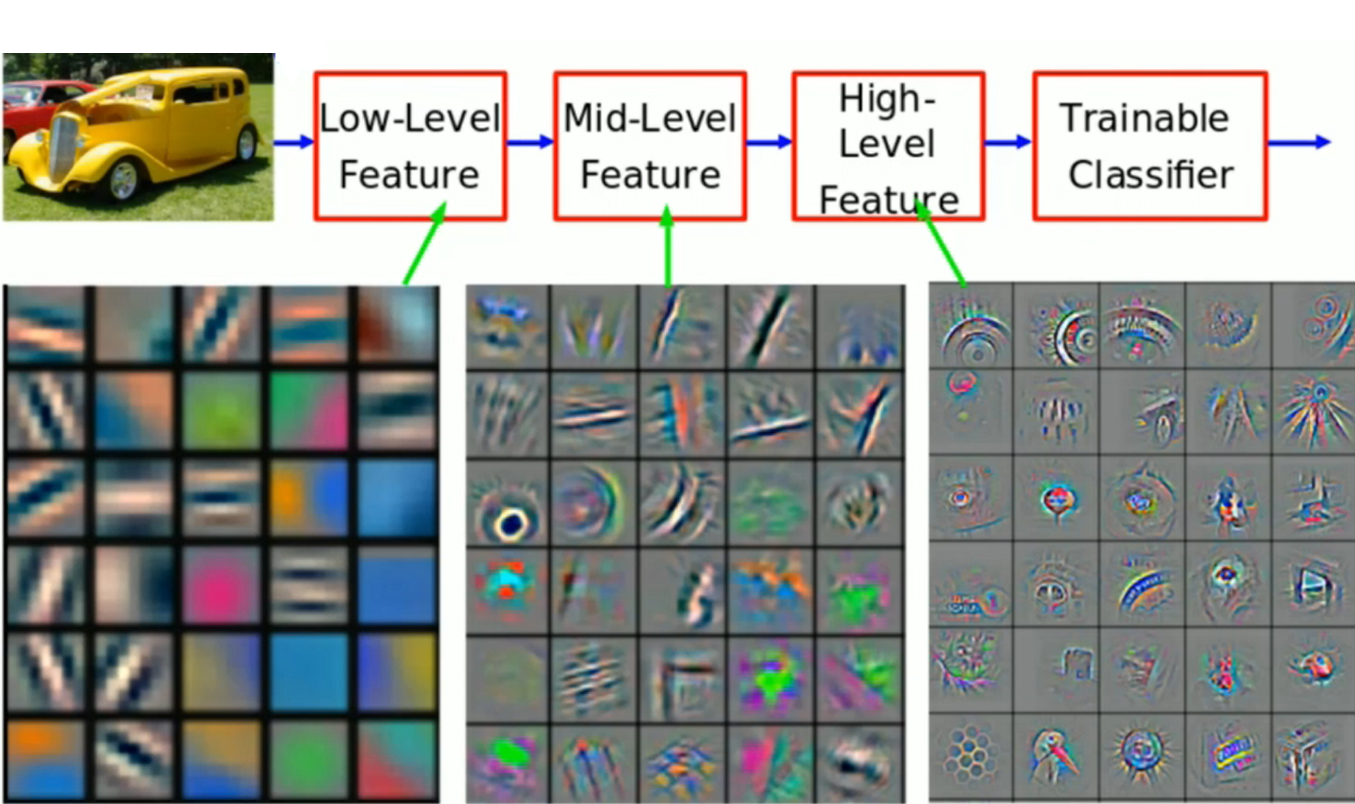
\includegraphics[width=0.5\textwidth]{lectures/03-b/images/FeatureExtraction.png}
\caption{An image of a car that has different levels of features extracted by different portions of a ConvNet.
Image taken from Professor LeCun's slides [Zeiler and Fergus].}
\end{figure}

This concept of learning progressively more complicated features is inspired from neurology and how the brain operates.
Specifically inspired from the ventral pathway in the visual cortex.
The area of the brain responsible for sight and sight processing.

In the 50s and 60s many scientists were curious with how the ventral pathway functions. 
It was shown that a specific neuron would `turn on', `fire', or `release neurotransmitter' when a straight edge was 
presented to the subject.
As that edge was rotated, the original neuron would turn off and a nearby neuron would turn on.
In addition, different neurons would turn on depending on the location of the edge in the input field.
So, clusters of neurons would be responsible for detecting an edge, and its orientation, in a specific location of the visual field.
These cells were designated with the term `simple cells' by Hubel and Wiesel.
Simple cells take input directly from the retina and detect local features.

Additionally it was noticed that some cells would turn on and stay turned on based on the input from these simple cells.
So, if an edge was placed in the visual field then moved some cells would continue to be turned on.
These cells were called complex cells by Hubel and Wiesel.
Complex cells that `pool' the outputs of simple cells within a retinotopic neighborhood into a more complex shape.
This pooling not only creates more complicated shapes it can also removes the locality of different features.

Engineers and scientists who had the capability decided to produce models similar to the ventral pathway.
Kunihiko Fukushima decided to make the neural-positron which mimicked this philosophy.
Layers of these neural-positrons were created and a complicated, biologically inspired learning algorithm was used.
This complicated, competitive learning algorithm was used as this was before backpropagation was created.
As neurons don't have `positive' or `negative' weights, there were inhibitory and excitatory neurons.
Lots of normalization factors as well as many tunable hyperparameters.
Nonetheless Fukushima created a working model.

Inspired by Hubel, Wiesel and Fukushima - Dr. LeCun came up with convolutional neural networks in the late 80s.
By taking these biologically inspired ideas and combining them with backpropagation trainable neural networks.
This was done on the MNIST character dataset and showed substantial results.
As this was a dark time, before the Internet, the only two datasets available with enough examples were the character dataset and 
the speech dataset.

\begin{figure}[ht]
  \centering    
      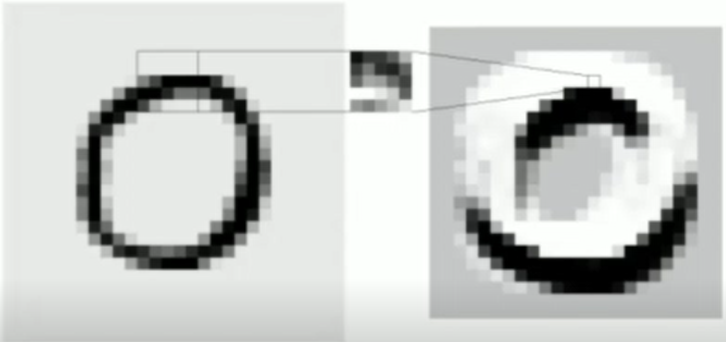
\includegraphics[width=0.5\textwidth]{lectures/03-b/images/ConvnetArch.png}
          \caption{
            A modern rendition of one layer in a convolutional neural network.
            The weighted sum, aka dot product, is taken between the filter and the input image.
            Input image on the left.
            5x5 filter, or kernel, in the middle.
            Output of the dot product on the right.
            White is a fully activated pixel.
            Black is a fully deactivated pixel.
            The output of the filter has been run through a non-linearity function ($\tanh$) that constrained the output to be between -1 and 1.
            This filter is useful for detecting horizontal edges.
            Image taken from Professor LeCun's slides.
          }
\end{figure}

A rendition of one layer of a convolutional neural network can be seen in Figure 7.2.
The dot product between the filter, or kernel, and the same size of the filter is conducted and that becomes a single pixel in the output image.
This filter is moved over the image one, or more, pixels at a time.
At each step the dot product is conducted between the input image and filter to produce a single pixel in the output image.
\href{https://cdn-images-1.medium.com/max/1600/1*ZCjPUFrB6eHPRi4eyP6aaA.gif}{As pictures are worth a thousand words click here to see a filter pass over an image.}

This is called a convolution.
Mathematically it's actually a cross correlation as a convolution subtracts the two values instead of adds them.
Regardless convolution is a better name.

\section{Architecture}
% Authors: Zach Tanenbaum, Taegyun Kim
% Lecture date: 2/11/2019

When a convolution is done over an image the size of the output image is smaller than the size of the input image.
If the input image is 100x100 and the filter is 3x3 then the resulting image will be 98x98.
This is because the 3x3 filter does not extend off of the input image so one pixel along the edge is lost.
If this is a big deal, padding can be used around the outside of the input image.
Typically the padding would be the mean of all pixel values in the image.

This shrinking of the image can be changed by using a different stride.
Stride is how many pixels to move the filter in between each step.

Backpropagation is used to train this filter for detecting specific features.
The values inside of the filter are considered weights to be learned.
Typically initialized to `random' or a modified random weights.
The typical structure for a convolutional neural network uses multiple layers of these filters before running the output of the last convolution layer through a fully connected neural network.
During training, the error is backpropagated through the fully connected neural network and then through the different filters.

This is a single filter runing over the image to produce an output.
The output of each filter is typically run through a non-linear function.
This non-linearity is used for the same reason non-linearity is used in a fully connected neural network.
As with a fully connected neural network ReLU or $\tanh$ are popular choices of non-linearity.
To allow the convolution layers to learn non-linear functions.
Typically multiple filters are run concurrently over a single input image to produce multiple output images.
The Conv2D module in PyTorch does all of this already.
God bless PyTorch.

Typically after a convolution layer there is a pooling layer.
Pooling layer shrink the image output from the convolution layer by a specified criteria.
On the pooling layer, a window is run over the image.
This window then takes the max, min, average or any other function between all pixels in the window.
So, if the window is 5x5 and max pooling is being conducted, the maximum value of the 5x5 grid is taken as a new pixel value.
The pooling layer creates a new, scaled down, image from the one provided.
Yes, PyTorch also has a max pooling module.
Yes, PyTorch is better than sliced bread.

\begin{figure}[ht]
  \centering
      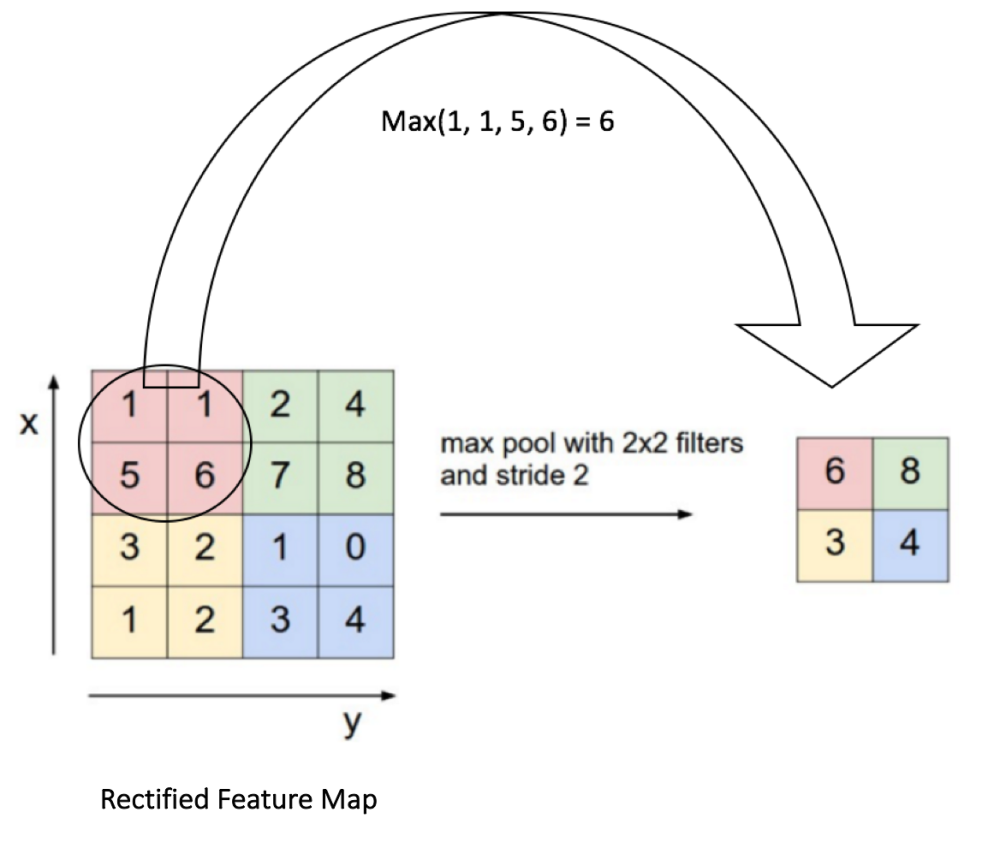
\includegraphics[width=0.5\textwidth]{lectures/03-b/images/MaxPooling.png}
          \caption{
            An example picture of how Max Pooling functions over an output from a Convolution Layer.
            \href{https://ulkarn.me/2016/08/11/intuitive-explanation-convnets/}{Source}
          }
\end{figure}

The reason pooling is used is to remove the localization on features.
If the pooling layer shrinks the input image by half then a feature would have to move two pixels before it is moved by one pixel in the output.
If another pooling layer shrinks the input image again by half then a feature would have to move four pixels in the original image to move one pixel in the output image.

Another popular version of pooling is the p-norm.
It allows the amount of pooling to be changed on the fly.
The equation for the p-norm is: $\Vert x\Vert _p = (\sum_{i=1}^{n} \|x_i\|^p)^{\frac{1}{p}}$.
When p is equal to one then it's just the L2 norm of the pixels.
When p is equal to infinity it's just max pooling.

After a convolution layer (with non-linearity) and a pooling layer another convolution layer (with non-linearity) can be run with a 3D filter.
This 3D filter takes the dot product of an area over multiple images.
This allows mutliple images to be condensed together into a single output.
As mentioned above, the first convolution layer could be run with mutliple filters that extract different features from an image and output images of those features.
So two filter can be used on an image to output an image of all vertical edges and all horizontal edges.
The 3D filter in this case could add all the vertical and horizontal edges together to determine all crosses in the picture.
PyTorch, thankfully has 3DConv layers.

\begin{figure}[ht]
  \centering
      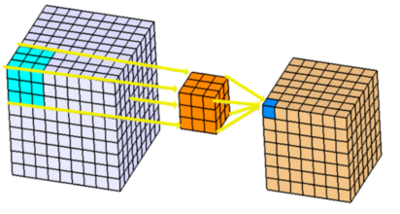
\includegraphics[width=0.5\textwidth]{lectures/03-b/images/3DConv.png}
          \caption{
            An example of a 3D filter condensing multiple images (on the left) into a new set of images on the right.
            If there were only 3 images on the left the resulting image would be a single image instead of a block of images.
            \href{https://www.kaggle.com/shivamb/3d-convolutions-understanding-use-case}{Source}
          }
\end{figure}

Mathematically, as each filter is looking at nearby pixels, nearby pixels need to be correlated.
Statistically, in natural images nearby pixels are correlated (remember cross correlation before?) and more often than not relate to a similar object.
In addition, uniform areas of an image are most frequent.
Then come edges between different areas of an image.
Lastly comes most other features.

Empirically, to save on computation costs, small kernels are typically used.
A 3x3 or 5x5 kernel requires dramatically less resources to run over an image than say a 17x17 kernel.
On a 100x100 image a 3x3 kernel will need to do 98x98 matrix multiplications between two 3x3 matrices for 86,436 computations.
On a 100x100 image a 5x5 kernel will need to do 96x96 matrix multiplications between two 5x5 matrices for 230,400 computations.
On a 100x100 image a 17x17 kernel will need to do 84x84 matric multiplications between two 17x17 matrices for 2,039,184 (a lot) computations.

Lastly, a normalization layer may be used to correct for image whitening.
A subtractive normalization layer may be used as a high pass filter.
A divisive normalization layer may be used to normalize the variance of the brightness aroudn the image.
This normalization layer is wholly optional.

So generally the overall architecture of a convolutional neural network has up to four different layers: Normalization, Convolution (aka Filter Bank), Non-Linearity and Pooling.
The general architecture for classification is Input Image $->$ Feature Extraction $->$ Fully Connected Neural Network $->$ Output Classification. 
Where the Feature Extraction can be any number of these blocks: Normalization (Optional) $->$ Convolution $->$ Non-Linear $->$ Pooling.

\begin{figure}[ht]
  \centering
      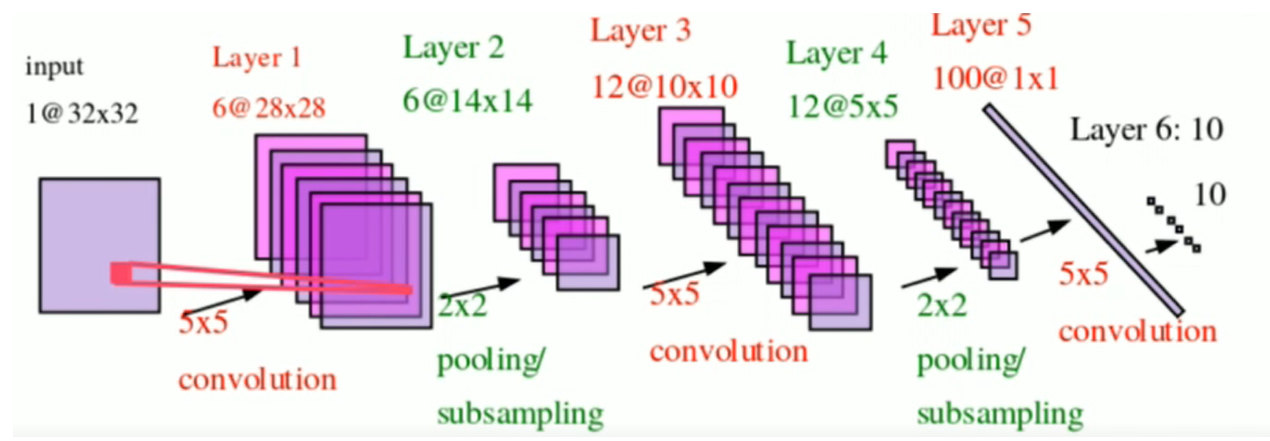
\includegraphics[width=0.5\textwidth]{lectures/03-b/images/PyTorchCNN.png}
          \caption{
            This is a convolutional neural network implemented in our lord and savior PyTorch with a graphical representation underneath.
            This network is used for digit recognition for the MNIST data set.
            This network was taken from Dr. Lecun's slides.
          }
\end{figure}

\begin{figure}[ht]
  \centering
      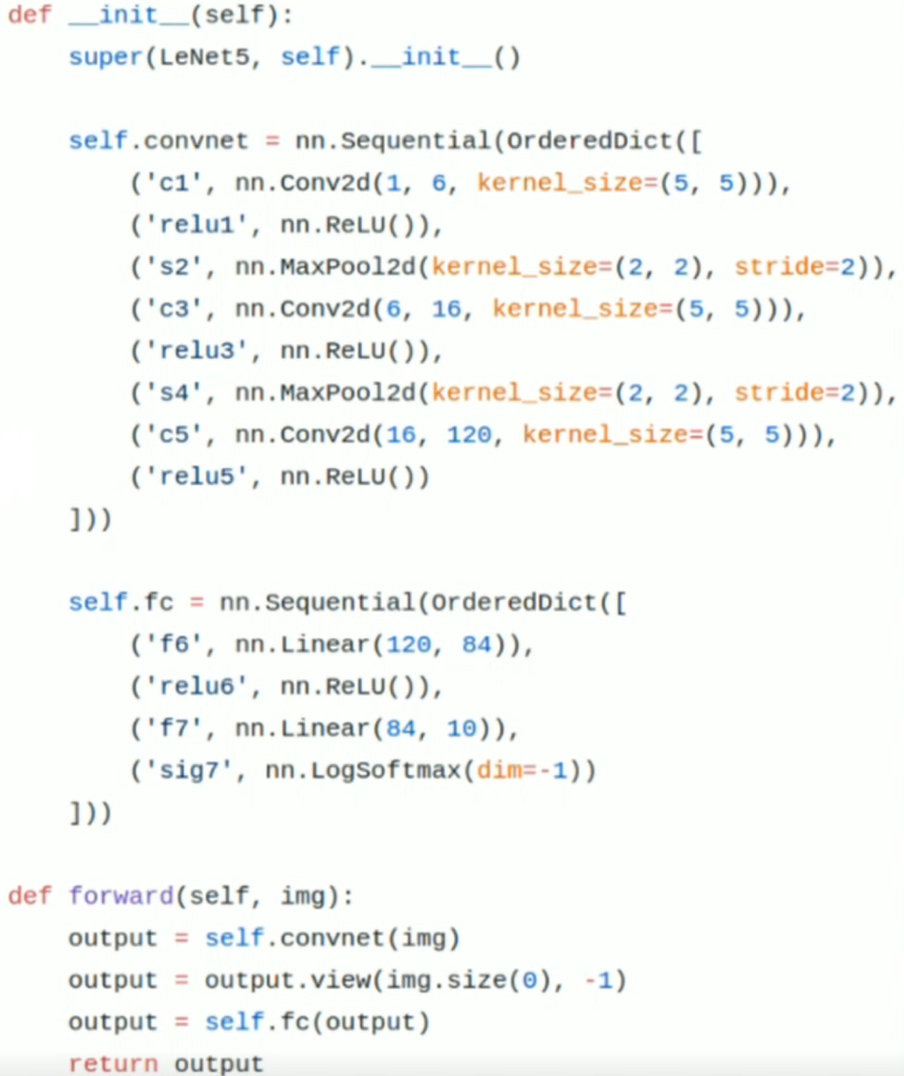
\includegraphics[width=0.5\textwidth]{lectures/03-b/images/PyTorchCNNSeq.png}
          \caption{
            This is (almost) the same convolutional neural network for solving the MNIST data set problem.
            In this case, the network is implemented in PyTorch (aka Better than Tensorflow) via the sequential object.
            This allows a network to be fully encompassed and easily transferrable.
            The main difference is that ReLU is used in this network instead of Tanh.
            This was also taken from Dr. Lecun's slides.
          }
\end{figure}

Now, one important aspect to convolutional neural networks is that the input can be variable. 
So, if a convolutional neural network is trained to recognize cursive letters no modification must be done to recognize a cursive sentence.
Traditionally, people would run the entire network on a section of the, now larger, input image.
Then move the entire network over and run it again on the next section of the input image.
With convolutional neural networks, the convolutional aspect of the network (not fully-connected portion) can be run over the whole image at once.
Then the fully connected portion can be moved over the slices of the output from the convolutional portion.
Running this fully-connected portion over the output layer can be though of as a convolution as well.
Where the input size is the same size as the kernel size and the stride is the same size as the width of the fully connected layer.
This significantly reduces computation of running a convolutional neural network over a larger image.
Initially, this ability to accept varying input sizes is was called a Space Discrepency Neural Network.

\begin{figure}[ht]
  \centering
      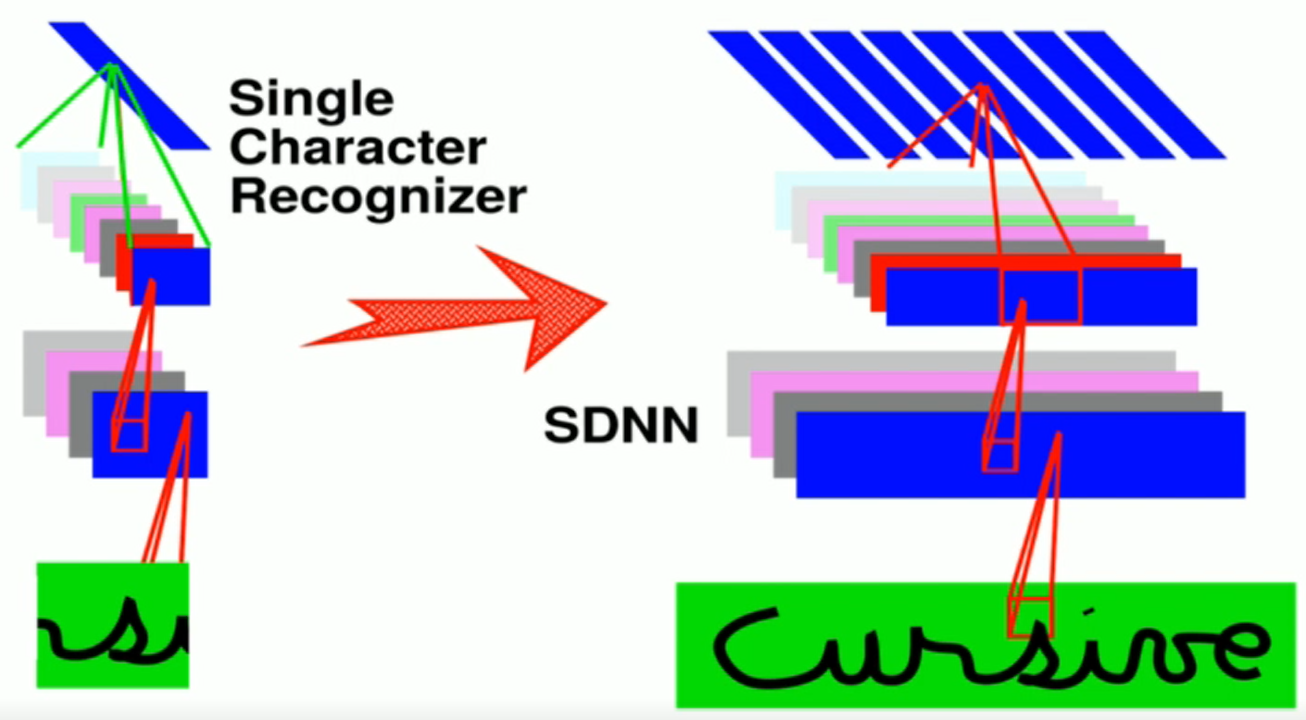
\includegraphics[width=0.5\textwidth]{lectures/03-b/images/SDNN.png}
          \caption{
            On the left is a convolutional neural network trained to recognize a single cursive character.
            On the right is the same network run over a larger input and the convolutional aspect fed segment by segment into the fully-connected portion.
            This image was taken from Dr. Lecun's slides.
          }
\end{figure}

There are ways to have a convolutional neural network view the overall image at once.
This technique is called 
Convolution Et Eau?.
This technique works by changing the stride size depending on the input.